\section{Problem Definition}
In this design scenario we look to understand the characteristics of the different properties of a heat exchanger. The team is given key constraints that limit the design. The affect of mass flowrate, number of tubes, and length of tubes will be varied and their affects will be studied. This counter-flow concentric-tube heat exchanger needs to heat 290K with supply waste water which is at 360K. The main constrains/specifications of the system are the following:
%
\begin{enumerate}
    \itemsep 0em 
    \item The length of each tube is not to exceed 10 m
    \item The outlet temperature of the hot water must be at least 10K higher than the inlet temperature of the cold water, namely, $T_{h,o} \geq 300K$
    \item The maximum number of tubes allowed is 8
    \item The waste hot water flow rate is 100 liters/minute
    \item Both the inner and outer tube diameters are held constant at 22mm and 45mm respectively
\end{enumerate}
%
%
\section{Single Tube Varying Mass Flowrate}
%
To first understand more about the design problem the team first studied a single pipe at constant length with the cold water flowing in the inner tube and the hot water in the outer tube annulus. The only variable varied in this experiment was the mass flowrate of the cold temperature stream. This provides insight into how the cold water flow has an effect on the outlet temperatures. The problem is formulated as the following:
%
\begin{equation} \label{eq_1}
    { C }_{ h }={ \dot { m }  }_{ h }{ C }_{ ph }\quad { C }_{ h }={ \dot { m }  }_{ c }{ C }_{ pc }\quad \rightarrow\quad { C }_{ r }=\frac { { C }_{ min } }{ { C }_{ max } } 
\end{equation}
%
\begin{equation} \label{eq_2}
    NTU=\frac { 1 }{ { R }_{ total }{ C }_{ min } } 
\end{equation}
%
To calculate this NTU value first the total resistance needs to be calculated for the heat exchanger. The thermal resistance circuit diagram can be constructed and drawn as the following:
%
\begin{figure}[H]
    \centering
    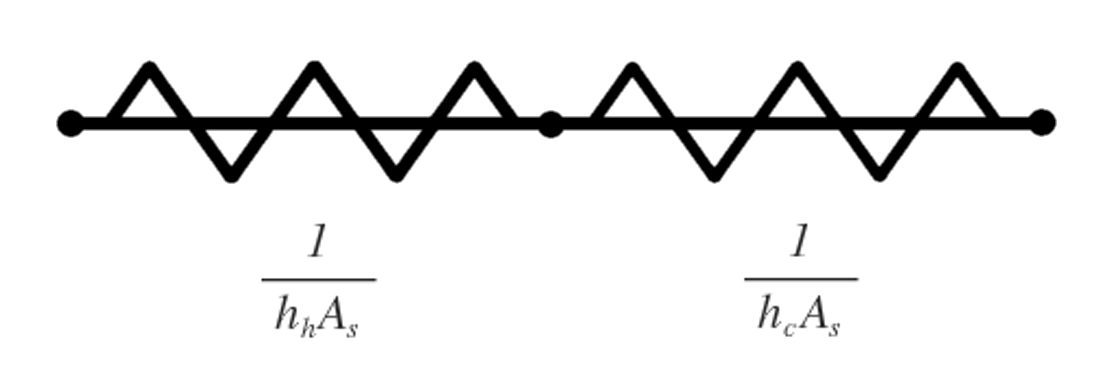
\includegraphics[width=3in]{pictures/part_1_total_resistance.png}
    \label{fig_part_1_1}
\end{figure}
%
\noindent
The internal pipe of the heat exchanger is taken to be ``very thin'', so the conduction though this pipe surface can be modeled as zero. The first step to finding the total resistance requires finding the convection coefficient for both the inner and outer surface of the heat exchanger. This requires the Reynolds number along with the Nusslet number for each surface. To calculate the Reynolds number we can use the equations below. It is important to note that the cross sectional area ${ A }_{ c }$ is different for the inner pipe and outer pipe (i.e. the outer pipe uses the hydraulic diameter, ${ D }_{ h }$, which is the difference between the outer diameter and the inner diameter.)
% Reynold numbers for pipes
\begin{subequations}
\begin{eqnarray}
 { Re }_{ D } =\frac { \rho { D }_{ i }{ V }_{ i } }{ \mu  } =\frac { { D }_{ i }{ \dot { m }  }_{ i } }{ \mu { A }_{ c } } \\ 
 { Re }_{ Dh } =\frac { \rho { D }_{ h }{ V }_{ i } }{ \mu  } =\frac { { D }_{ h }{ \dot { m }  }_{ o } }{ \mu { A }_{ c } } 
\end{eqnarray}
\end{subequations}
%
It is important to note that the diameter used for the outer tube, ${ D }_{ h }$, used the hydraulic diameter which is the difference between the outer diameter and the inner diameter. Once the Reynolds number is known for both parts, the Nusslet number can then be calculated using the equations below. 
%
% Inner tube
\begin{subequations}
\label{eq_part_1_5}
\begin{eqnarray}
 { R }e_{ D }<3000:\quad { Nu }_{ D }=4.36 \\
 { R }e_{ D }>3000:\quad { Nu }_{ D }=0.023{ Re }_{ D }^{ 0.8 }{ Pr }^{ n } 
\end{eqnarray}
\end{subequations}
% Outer tube
\begin{subequations}
\label{eq_part_1_6}
\begin{eqnarray}
 { R }e_{ Dh }<3000:\quad { Nu }_{ Dh }=5.74 \\
 { R }e_{ Dh }>3000:\quad { Nu }_{ Dh }=0.023{ Re }_{ Dh }^{ 0.8 }{ Pr }^{ n } 
\end{eqnarray}
\end{subequations}
%
Where the following is true for both n values:
%
\begin{equation}
 n=\left\{ \begin{matrix} 0.3\quad if\quad { T }_{ s }<{ T }_{ m } \\ 0.4\quad if\quad { T }_{ s }>{ T }_{ m } \end{matrix} \right\} 
\end{equation}
%
%
Equations \eqref{eq_part_1_3} was then used to find the convection coefficient for each tube. Once both \textit{h}'s were found, the total resistance of the system could be calculated using \eqref{eq_part_1_4} below, where the surface area is the surface area of the inner pipe.
% Convection coefficent calculation
\begin{subequations}
\label{eq_part_1_3}
\begin{eqnarray}
 { \bar { h }  }_{ i }=\frac { { Nu }_{ D }{ k }_{ fluid } }{ { D }_{ i } }  \\
 { \bar { h }  }_{ o }=\frac { { Nu }_{ Dh }{ k }_{ fluid } }{ { D }_{ h } }  
\end{eqnarray}
\end{subequations}
%
\begin{equation}
 \label{eq_part_1_4}
 { R }_{ total }=\frac { 1 }{ { \bar { h }  }_{ i }{ A }_{ s } } +\frac { 1 }{ { \bar { h }  }_{ o }{ A }_{ s } } 
\end{equation}
%
Following the calculation of total resistance, the minimum and maximum capacity rate needed to be calculated, as seen in equation \eqref{eq_1}, which is used to determine the NTU value as stated above. Along with the $C_{min}$ and $C_{max}$ value, the $C_{r}$ is needed to find the heat exchanger effectiveness which can be found using \eqref{eq_1} from above. To find the heat exchanger effectiveness equation \eqref{eq_3} was used. Then with the application of equation \eqref{eq_4} the rate of heat transfer of the system can be determined.
%
\begin{equation} \label{eq_3}
\varepsilon =\frac { 1-exp\left( -NTU\left( 1-{ C }_{ r } \right)  \right)  }{ 1-{ C }_{ r }{ exp\left( -NTU\left( 1-{ C }_{ r } \right)  \right)  } } 
\end{equation}
%
\begin{equation} \label{eq_4}
 q=\varepsilon { C }_{ min }\left( { T }_{ h,i }-{ T }_{ c,i } \right) 
\end{equation}
This can then be applied to energy balance where the outlet temperatures vary based on the different mass flowrates. We can then find both the hold and cold outlet temperatures of the system. This entire process can be repeated for a different cold mass flowrate and the results can be compared. The results can be seen below.
%
\begin{subequations}
\begin{eqnarray}
 q={ C }_{ c }\left( { T }_{ c,o }-{ T }_{ c,i } \right)  \\
 q={ C }_{ h }\left( { T }_{ h,i }-{ T }_{ h,o } \right) 
\end{eqnarray}
\end{subequations}
%
\begin{figure}[H]
    \centering
    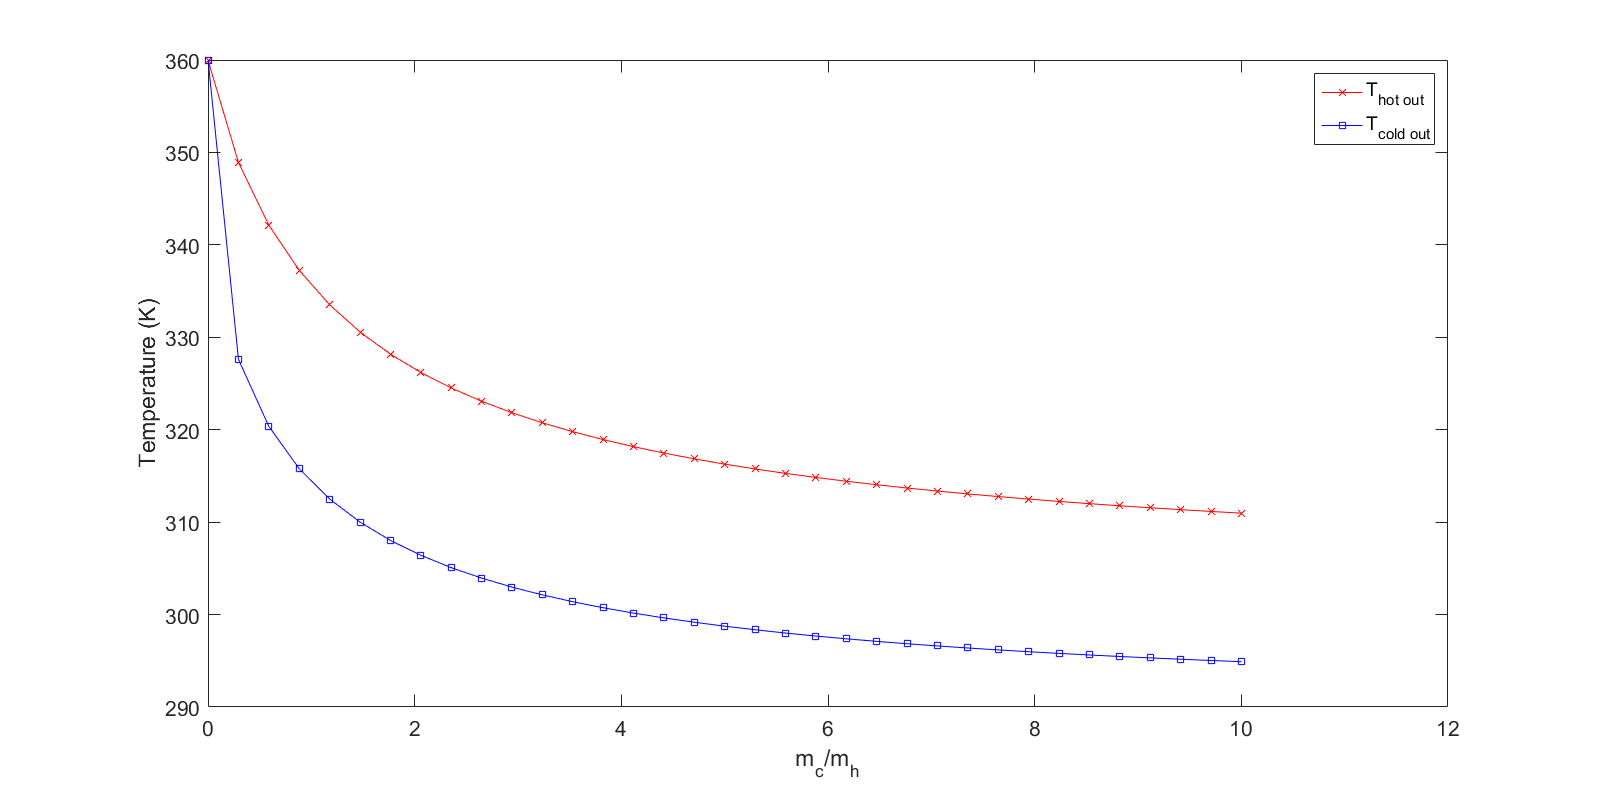
\includegraphics[height=3.5in]{pictures/part_1_temp_out.png}
\end{figure}
%